%% Template for a preprint Letter or Article for submission
%% to the journal Nature.
%% Written by Peter Czoschke, 26 February 2004
%%

\documentclass{natureJMK}

\usepackage{graphicx}
\usepackage{bkdefs}
\usepackage[plain]{fancyref}
\usepackage{lineno}
\renewcommand*{\Freffigname}{Fig.}
\renewcommand*{\freffigname}{Fig.}

%% make sure you have the nature.cls and naturemag.bst files where
%% LaTeX can find them
\newcommand{\tempS}[1]{}

\bibliographystyle{naturemag}
\linenumbers
\title{Submesoscale streamers exchange water on the north wall of the Gulf Stream}

%% Notice placement of commas and superscripts and use of &
%% in the author list

\author{Jody M. Klymak$^{1}$, R. Kipp Shearman$^2$, Jonathan Gula$^3$, Craig M. Lee$^4$, Eric A. D'Asaro$^4$, Leif N. Thomas$^5$, Ramsey Harcourt$^4$, Andrey Shcherbina$^4$, Miles A. Sundermeyer$^6$, Jeroen Molemaker$^7$ \& James C. McWilliams$^7$}

\begin{document}

\maketitle

\begin{affiliations}
 \item University of Victoria, Victoria, British Columbia, Canada
 \item Oregon State University, Corvallis, Oregon, USA
 \item Laboratoire de Physique des Oc\'eans, Universit\'e de Bretagne Occidentale, Brest, France
 \item Applied Physics Laboratory, University of Washington, Seattle, Washington USA
 \item Stanford University, Stanford, California, USA
 \item University of Massachusetts Dartmouth, Dartmouth, Massachusetts, USA
 \item University of California, Los Angeles, California, USA 
\end{affiliations}

\begin{abstract}
The Gulf Stream is a major conduit of warm surface water from the tropics to the subpolar North Atlantic.  Its north side has a strong  temperature and salinity front that is maintained for hundreds of kilometers despite considerable energy available for mixing.  Large mesoscale ($\mathbf{>20}$ km) ``rings'' often pinch off, but like the Gulf Stream they are resistant to lateral mixing, and retain their properties for a long time.  Here we observe and simulate a sub-mesoscale ($\mathbf{<20}$ km) mechanism by which the Gulf Stream exchanges water with the cold subpolar water to the north. A series of ``streamers'' detrain partially mixed water from the Gulf Stream at the crest of meanders. Subpolar water is entrained replacing the partially mixed water, and helping to resharpen the front. The water mass exchange can account for a northwards flux of salt of $0.8-5\ \mathrm{psu\ m^2s^{-1}}$, which can be cast as an effective local diffusivity of $O(100\ \mathrm{m^2s^{-1}})$. This  is similar to bulk-scale flux estimates of $1.2\ \mathrm{psu\ m^2s^{-1}}$ and is enough to supply  fresh water to the Gulf Stream as required for the production of 18-degree subtropical mode water. 
\end{abstract}

The Gulf Stream (GS) is the western boundary current of the North Atlantic subtropical wind-driven circulation.  It separates from Cape Hatteras and extends into the interior North Atlantic, traveling east.  As it does so, it loses heat not only to  the atmosphere, but also by mixing with the cold water in the subpolar gyre to the north.  It also becomes fresher, an observation that can only be explained by entrainment of fresh water from the north \cite{joyceetal13}.  As it entrains water, the GS  increases its eastward transport by approximately $4-8\times 10^6 \mathrm{m^3s^{-1}}$/100 km (Johns et.\ al.\\cite{johnsetal95}).   A sharp density front creates thermal wind shear that confines the current to the upper ocean.  

The north wall of the GS has a very sharp temperature-salinity front, even along constant-density surfaces.  Salinity decreases by almost 1.5 psu looking north along isopycnals, corresponding to a drop in temperature of $5\mathrm{^oC}$.   The sharpness of this front persists for 100s of kilometers, despite the fact that mixing along isopycnals is much easier than across them. However, the GS water has a very high potential vorticity gradient (angular momentum; see methods) that is believed to act as a barrier to mixing on large scales \cite{marshalletal06,naveiraetal11}.  

Despite this  barrier and the presence of the sharp front, budgets of properties of the GS indicate that there is significant exchange across the north wall\cite{joyceetal13}.  Entrainment of fresh water is necessary to create the dynamically important ``18-degree water'' that fills much of the upper Sargasso Sea. There are large eddies that periodically pinch off the GS and carry warm water to the north. However, some of these are re-entrained into the GS and do not result in a net exchange. Instead, tracer budgets across the front appear to be dominated by small-scale processes\cite{boweretal85}. To date some of the best direct evidence for cross-front exchange consists of the trajectories of density-following floats placed at the north wall \cite{bowerrossby89,bowerlozier94}.  These floats were observed to regularly detrain from the GS, such that of 95 floats, 26 stayed in the GS, 7 were detrained in rings, and 62 were detrained by mechanisms other than rings\cite{bowerlozier94}.  Some floats that detrained were also observed to move upwards rapidly.  Kinematic theories have been examined to explain the detrainment of the floats \cite{flierletal87,stern85}, but direct observations of the relevant processes have been lacking.  

%TODO: Make these paras shorter
% The streamers carry  warm, salty, and high-vorticity  water north of the stream.  Because they have cyclonic vorticity anomaly, they also wrap up cold fresh water and entrain it into the GS\cite{stern85}.  The preferential detrainment of partially mixed water helps explain the persistent sharpness of the GS front despite the presence of mixing processes at the base of the GS.  We also speculate that the preferential detrainment of this water into the streamers is dynamically linked to the partial mixing of vorticity at the base of the GS. 

Here we present evidence that there is small-scale mixing ($<$0.5 km)  on the northern cyclonic side of the GS, and that the partially mixed water periodically peels off the GS in thin (5-10 km wide) ``streamers''.  In March 2012 we made high-resolution measurements of the north wall of the GS from 66 W to 60 W (\fref{fig:SatOverviewSectD}), about 850 km east of where the GS separates from the North American continental slope.  Two research vessels tracked a water-following float placed in the GS front and programmed to follow the density of the surface mixed layer. The float was transported downstream with a relatively constant speed of 1.4 $\pm 0.2 \mathrm{m\,s^{-1}}$, in water that became denser  as the surface of the GS cooled.  One vessel maintained tight sampling around the float and deployed an undulating profiler to 200 m, making 10-km cross sections every 10 km downstream.  The second vessel  had an undulating profiler making larger 30-km  scale sections.  Both profilers measured temperature, salinity and pressure, and had approximately 1-km along-track resolution; both ships also measured ocean currents.  Fluorescent dye was deployed near the floats on some deployments, and measured by the profilers on the ships. By following the float, a focus on the front was maintained as it curved and meandered to the east.  

During these observations, the GS had a shallow meander crest at 65 W (\fref{fig:SatOverviewSectD}b)  followed by a long concave region (63 W) and then another large  crest (61 W).  Satellite measurements show the sharp temperature changes across the front, superimposed with thin intermediate-temperature (15-18$^o$C) streamers detraining to the north at approximately 65 W, 64 W, and at the crest of the large meander at 61 W.  An older streamer that has rolled up can also be seen at 62 W.  The ships passed through the three newer streamers providing the first detailed observations of their underwater structure.  

The front consists of density surfaces that slope up towards the north (\fref{fig:SalDFirstStreamer}a-d).  The water along the density surfaces is saltier (and warmer) in the GS, and fresher (and colder) to the north.  The temperature-salinity (T/S) relationship shows the contrast between the two water masses as two distinct modes (\fref{fig:ComposeTSfigNew}a), except near the surface where the water masses are strongly affected by the atmosphere.  There is a third population between the two larger modes in T/S space that we identify as the streamers.  In the cross-sections, these are the intermediate salinity anomalies ($S \approx 36.15\ \mathrm{psu}$; \fref{fig:SalDFirstStreamer}a--d).  Along $\sigma_{\theta}=26.25\ \mathrm{kg\,m^{-3}}$, these anomalies are horizontally connected, peel off the north wall of the GS, are 5-10 km wide, and  stretch for almost 50 km along the wall (\fref{fig:ComposeTSfigNew}b). The streamers have a strong positive potential vorticity signature.  Along the $26.25 \ \mathrm{kg\,m^{-3}}$ isopycnal, the region of high potential vorticity corresponds very well with the partially mixed streamer water (\fref{fig:SalDFirstStreamer}i--l, \fref{fig:ComposeTSfigNew}b ).   

The streamers remove water from the main GS flow.  The velocity contrast across the front is  sharp, with $>1\ \mathrm{m\,s^{-1}}$ drop in 5 km (\fref{fig:SalDFirstStreamer}e--h, \fref{fig:ComposeTSfigNew}b ).  The streamers start on the fast side of the front, moving approximately $0.25\ \mathrm{m\,s^{-1}}$ faster than the float (\fref{fig:SalDFirstStreamer}h). Upstream, where they are detached (\fref{fig:SalDFirstStreamer}e), they are moving almost $0.5\ \mathrm{m\,s^{-1}}$ slower than the float.  This represents a considerable detrainment from the GS.  A 5-km wide and 150-m deep streamer, detraining with a relative velocity of $0.75\ \mathrm{m\,s^{-1}}$ represents a rate of detrainment of over $0.5\times10^{6}\, \mathrm{m^{3}\,s^{-1}}$.  

The streamers move up through the water column along isopycnals and the water parcels are stretched vertically. The streamer in \fref{fig:SalDFirstStreamer}a has risen along isopycnals from 140 m deep (\fref{fig:SalDFirstStreamer}d)  to less than 40 m deep, and titled somewhat as it has done so.   The velocity anomaly is about $0.75\ \mathrm{m\,s^{-1}}$ over 100 km so we estimate that the streamer is approximately 1.5 days old,  implying vertical velocities of order  50 m/day, similar to rates inferred from large-scale omega-equation calculations\cite{thomasjoyce10}.  

Concurrently, there is an acceleration of fresh water from the north that is enfolded between the streamers and the GS, which we will call an ``intrusion''. The acceleration of the intrusion is hard to quantify in the sections above because it is drawn from a large pool of water upstream.  However, a subsequent survey of the north wall (March 14) included a dye release in this reservoir that was then entrained in an intrusion (\fref{fig:StreamersModel}a-c). The streamer during this occupation was less pronounced than the one described above, but was clear for a number of passes through the north wall.  The dye cloud was quite spread out, but the data show clear interleaving of the intrusion water.  

High-resolution numerical simulations ($dx\approx 500 m$, see Methods) resolve these features and also confirm the entrainment of the fresh intrusion (\fref{fig:StreamersModel}d-i). Seeding the simulation with Lagrangian particles (see methods) allows us to track the evolution of the streamers and the intrusion as the flow moves downstream.  Before the streamer is formed, the water in the intrusion (magenta contours) is near the surface and the streamer water (green contours) is well within the front (\fref{fig:StreamersModel}d,g).  Downstream (\fref{fig:StreamersModel}e,h) the fresh water has been subducted to 150 m depth, and the streamer has been pushed north of the front.  Both water masses accelerate with the whole GS between these two snapshots (\fref{fig:StreamersModel}f), but the fresh intrusion accelerates more, such that the intrusion is entrained and the streamer slows and is detrained.  As in the observations, the streamer occupies an intermediate region in T-S space (\fref{fig:StreamersModel}i, green contour), and originates in the high-vorticity region of the front.   

The acceleration of the fresh intrusion relative to the streamer is an important finding of the model, as the fresh water now forms a new sharp T-S front with the warm salty GS, and the partially mixed streamer water is carried away from the front.  The model further shows that the streamers are more prominent on the leading edges of meanders, also clearly seen in satellite images (\fref{fig:SatOverviewSectD}).  There are differences with the observations, however.  The data show very distinct T-S signatures associated with the streamers, whereas the model streamer T/S ``mode'' is less isolated (\fref{fig:StreamersModel}i).  The two interleaving water masses are   confined to a narrow isopycnal band in the model, with the intrusion being slightly lighter than the streamer, whereas in the observations the temperature-salinity front cuts across more isopycnals (compare \fref{fig:SalDFirstStreamer}b to \fref{fig:StreamersModel}h).   There is also clear evidence of strong subduction of the intrusion in the model, reminiscent of intrathermocline eddies \cite{thomasjoyce10}.    

Differences between the data and the model aside, there are two major implications of the loss of partially mixed water to the north.  The first is that it helps explain why the front at the north wall of the GS remains so sharp.  It is not that there is no mixing taking place in both the horizontal and the vertical, but rather that the mixing product is carried away in the streamers.  It is striking that it is only partially mixed water that is carried away, and not high-salinity GS water (\fref{fig:ComposeTSfigNew}b), and that this is also high-vorticity water.  This implies a dynamical link that we have not seen explored.  Streamers have been observed from surface temperature in satellites and floats\cite{bowerrossby89,flierletal87,lozieretal97,songetal95}, and this has led to kinematic models in which particles are displaced from streamlines going around propagating meanders \cite{bower91,prattetal95,lozieretal97}. The observations here add to these models by showing that it is only partially mixed water that leaves the GS.  This co-incidence indicates to us a role for small-scale mixing in producing the destabilizing forces that cause this water to detrain from the north wall.  The observations and simulation indicate that the meanders of the GS play an important role in the formation of the streamers.

The second implication is that the streamers are a mechanism that can balance large-scale budgets that require significant exchange across the GS\cite{joyceetal13,boweretal85}. Such budgets suggest that this region of the GS loses salinity to the north at a rate of $1.2\ \mathrm{psu\  m^2 s^{-1}}$ \cite{joyceetal13}.  Each streamer transports $0.2-0.5 \times 10^6\ \mathrm{m^3 s^{-1}}$ of water that is $0.8-1\ \mathrm{psu}$ saltier than the water that is entrained.  Streamers appear approximately every 100-300 km, associated with meanders, so an estimate of their average transport is $0.8-5\ \mathrm{psu\ m^2s^{-1}}$, bracketing the large-scale estimates.  Working against a gradient of 1 psu/10 km over 200 m depth, the equivalent lateral diffusivity is $40-250\ \mathrm{m^2s^{-1}}$. More observations would need to be made to make this transport estimate more robust.

Here we have observed a lateral stirring process along the north wall of the GS.  Small-scale mixing due to a number of possible processes\cite{thomasshakespeare15,whittthomas13} at the north wall temperature-salinity front creates an intermediate mass of water that, if it accumulated, would weaken the sharpness of the front. However,  streamers detrain the partially mixed water, and entrain cold and fresh water toward the north wall, resharpening  the temperature-salinity front.  An alternative possibility is that partially mixed water is squeezed by frontogenetic strain, but such squeezing would require  this water to move downstream.  Given the length of the GS, either the intermediate water must accelerate, or  there is an accumulation somewhere downstream. Given that there is no strong evidence of either large-scale  acceleration, nor a place where this water mass accumulates, the streamers are a viable mechanism that removes this the mixing product.  


\section{Methods}

The Lagrangian float was placed in the Gulf Stream front based on a brief cross-stream survey, and programmed to match the density of the surface mixed layer (upper 30 m).  The float moved downstream at a mean speed of 1.4 $\mathrm{m\,s^{-1}}$.  The \emph{R/V Knorr} tracked the float and deployed a Chelsea Instruments TriAxus that  collected temperature, salinity, and pressure (CTD) on a 200-m deep sawtooth with approximately 1-km lateral spacing in a 10-km box-shaped pattern relative to the float (\fref{fig:SatOverviewSectD}, magenta).  \emph{R/V Atlantis} maintained a larger set of cross sections approximately 30 km across the front, trying to intercept the float on each front crossing.  \emph{R/V Atlantis} was deploying a Rolls Royce Marine Moving Vessel Profiler equipped with a CTD that profiled to 200 m approximately every 1 km.  Both ships had a 300 kHz RDI Acoustic Doppler Current Profiler (ADCP) collecting currents on 2-m vertical scale averaged every 5 minutes (approximately 1 km lateral scale), collected and processed using UHDAS and CODAS (http://currents.soest.hawaii.edu\cite{firingetal12}).  This data reached about 130 m, and was supplemented at deeper depths with data from 75 kHz RDI ADCPs, with 8-m vertical resolution.  

Data were interpolated onto depth surfaces by creating a two-dimensional interpolation onto a grid via Delauney triangulation. No extrapolation was performed.  Data on the $26.25\ \mathrm{kg\,m^{-3}}$ isopycnal were assembled at each grid point by finding the first occurrence of that isopycnal in depth.  

Potential vorticity is calculated from the three-dimensional grid as
\begin{equation}
  q = -\frac{g}{\rho_0}\left(\nabla \times\mathbf{u}+\mathbf{f}\right) \cdot \nabla\rho,
\end{equation}
where $f$ is the Coriolis frequency, $g$ the gravitational acceleration. The bracketed term is twice the angular velocity, including the planet's rotation, and the gradient of density represents the stretching or compression of the water column.  In the GS, the potential vorticity is dominated by contributions from the vertical density gradient and the cross-stream gradient of the along-stream velocity:
\begin{equation}
  q \approx N^2\left(-\frac{\partial u}{\partial y}+f\right).
\end{equation}

Dye Release. At select times during the float evolutions, fluorescein dye releases (100 kg per release) were conducted at depth as close as possible to the float.  Dye was pumped down a garden hose to a tow package deployed off the side of the ship, consisting of a CTD and a dye diffuser.  Prior to injection, the dye was mixed with alcohol and ambient sea water to bring it to within $0.001\ \mathrm{kg m^-3}$ of the float's target density. Initial dimensions of the dye streak were $\approx$1 km along-stream, $\approx$100 m cross-stream (after wake adjustment), and ranging from 1 - 5 m in the vertical. The TriAxus system on the \emph{R/V Knorr} tracked the fluorescein from its CTD package.  

Numerical simulation. The high-resolution realistic simulation of the GS is performed with the Regional Oceanic Modeling System (ROMS\cite{shchepetkinmcwilliams05}). This simulation has a horizontal resolution of 500m and 50 vertical levels. The model domain spans 1,000 km by 800 km and covers a region of the GS downstream from its separation from the U.S. continental slope. Boundary conditions are supplied by a sequence of two lower-resolution simulations that span the entire GS region and the Atlantic basin, respectively. The simulation is forced by daily winds and diurnally modulated surface fluxes. The modelling approach is described in detail in Gula et.\ al\cite{gulaetal15}.

Virtual Lagrangian Particles.  The neutrally buoyant Lagrangian (flow-following) particles were seeded at time 285 and advected both backwards and forwards from this time by the model velocity fields without  additional dispersion from the model's mixing processes\cite{gulaetal14}. A 4th-order Runge-Kutta method with a  time step  $dt = 1\ \mathrm{s}$ is used to compute particle advection. Velocity and tracer fields are interpolated at the positions of the particles using cubic spline interpolation in both the horizontal and vertical directions.  We use hourly outputs from the simulation to get sufficiently frequent and temporally-smooth velocity sampling for accurate parcel advection.



%% Put the bibliography here, most people will use BiBTeX in
%% which case the environment below should be replaced with
%% the \bibliography{} command.

\bibliography{main}

%\begin{thebibliography}{1}
%\bibitem{dummy} Articles are restricted to 50 references, Letters
%to 30.
%\bibitem{dummyb} No compound references -- only one source per
%reference.
%\end{thebibliography}


%% Here is the endmatter stuff: Supplementary Info, etc.
%% Use \item's to separate, default label is "Acknowledgements"


\clearpage
\listoffigures
\clearpage

\begin{addendum}
 \item  Our thanks to the captains and crews of \emph{R/V Knorr} and \emph{R/V Atlantis}, The AVHRR Oceans Pathfinder SST data were obtained from the Physical Oceanography Distributed Active Archive Center (PO.DAAC) at the NASA Jet Propulsion Laboratory, Pasadena, CA. http://podaac.jpl.nasa.gov. Funding was supplied by Office of Naval Research, Grants XXXXXX
 \item[Competing Interests] The authors declare that they have no
competing financial interests.
 \item[Correspondence] Correspondence and requests for materials
should be addressed to Jody M. Klymak.~(email: jklymak@uvic.ca).
\end{addendum}
\clearpage

\begin{figure*}[htbp]
  \centering
    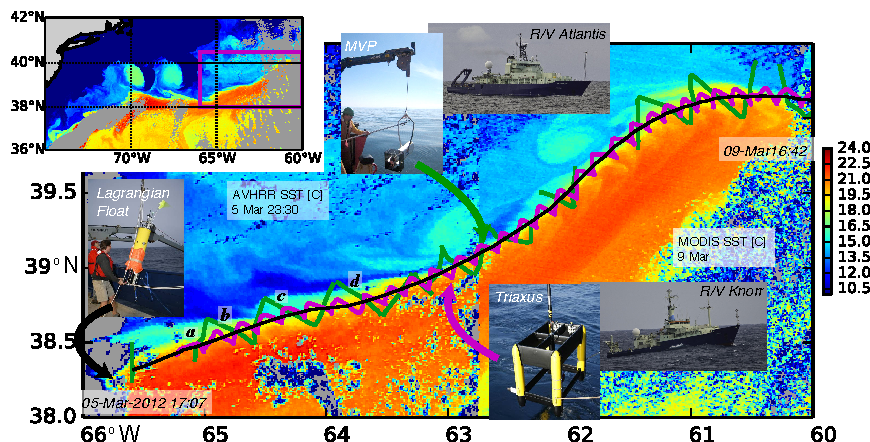
\includegraphics[width=\textwidth]{./SatOverviewSecDTry2.pdf}
   \caption{{\bf Experimental design.}  Inset: The experiment site on the north wall of the Gulf Stream, between 66 and 60 W, as shown in an AVHRR satellite image of sea surface temperature (SST).  Main:  Detailed SST image composed from two satellites images.    The GS is warm and delineated by a sharp front.  There are small sub-mesoscale structures north of the front, which are the focus of this paper.  The satellite images are a composite from early in the observation period (AVHRR 6 Mar), and late (MODIS, 9 Mar).  A Lagrangian float was deployed in the front (black curve), and the ship tracks bracketed the float's position (green: \emph{R/V Atlantis}, magenta: \emph{R/V Knorr}). \emph{R/V Atlantis} cross-sections labeled a-d are shown in \fref{fig:SalDFirstStreamer}a-d.  }\label{fig:SatOverviewSectD}
\end{figure*}

\begin{figure*}[htbp]
  \centering
    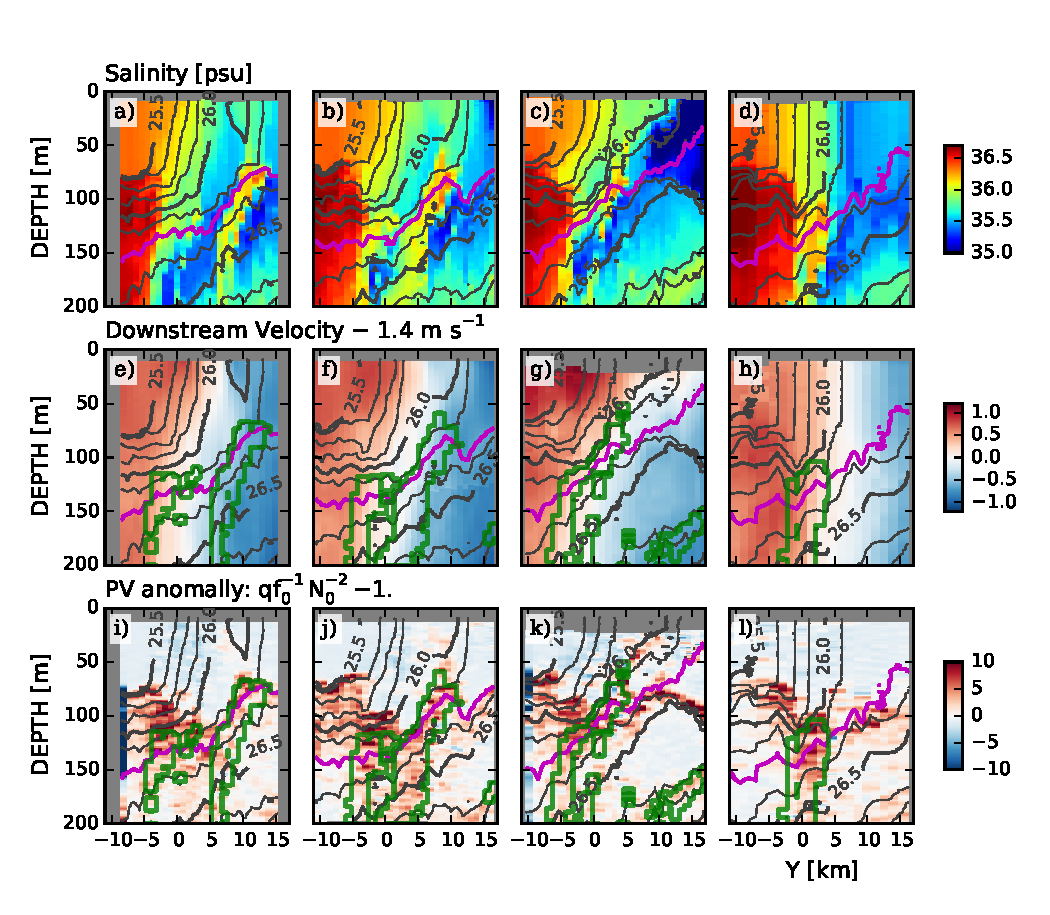
\includegraphics[width=\textwidth]{./SalDFirstStreamer.pdf}
    \caption{{\bf Cross sections of data collected across the Gulf Stream.}   $Y$ is the cross-stream distance perpendicular to the path of the float, positive being northwards.  The four columns correspond to the  four sections labeled a-d in \fref{fig:SatOverviewSectD}. Potential density is contoured in black and $\sigma_{\theta}=26.25\ \mathrm{kg\,m^{-3}}$ is magenta.  Along a constant density surface salty water is warmer than fresher water, so the GS on the left is warm and salty.  Section a) is the furthest upstream section (65W) and d) is the furthest downstream (63.75 W) (\fref{fig:ComposeTSfigNew}b).  e)--h) downstream velocity calculated relative to the float's trajectory by removing the float's mean speed of $u_{float}=1.4\ \mathrm{m\,s^{-1}}$ for the observation period.   Green contours are regions in temperature-salinity space labeled ``streamers'' in \fref{fig:ComposeTSfigNew}a.  i)--l) Potential vorticity sections (see text);
 } \label{fig:SalDFirstStreamer}
\end{figure*}


\begin{figure*}[htbp]
  \centering
    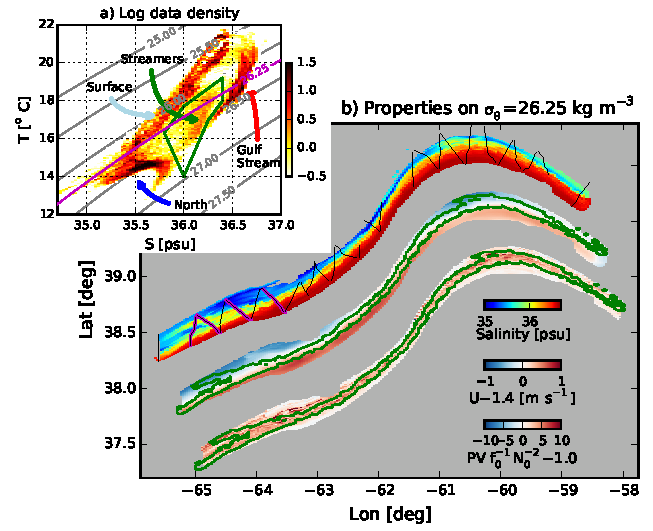
\includegraphics[width=0.9\textwidth]{./ComposeTSfigNew.pdf}
  \caption{{\bf Streamer properties and distribution in space.}
a) Logarithmically scaled histogram
 in temperature-salinity space (colours). The warm-salty GS water is very distinct from the water to the north, which is cold and fresh.  The water near the surface is heavily modified by the atmosphere.  Deeper, there is a class of water distinct from the GS water and the water to the north, that we label ``streamers''.  This water is contoured in green in \fref{fig:SalDFirstStreamer}e-l.  b) Interpolation of salinity, velocity, and potential vorticity onto the $\sigma_{\theta}=26.25\ \mathrm{kg\,m^{-3}}$ isopycnal, plotted geographically (with a small exaggeration of scale in the north-south direction, and the latter two fields offset slightly to the south-east). This used data from both ships.  The ship track for the \emph{Atlantis} is plotted in black, and the four cross-sections in \fref{fig:SalDFirstStreamer} are plotted in magenta.  The streamer water is contoured in green.  
  } \label{fig:ComposeTSfigNew}
\end{figure*}

\begin{figure*}[htbp]
  \centering
    \includegraphics[width=0.9\textwidth]{./dye_ts.pdf}
    \includegraphics[width=0.9\textwidth]{./model.pdf}
  \caption{{\bf Evidence for entrainment of intrusions from a dye release and numerical simulation.}
a) Salinity section from an occupation of the GS 14 March. The location of a dye is contoured in magenta.  b) Salinity section from downstream.  A streamer has enfolded the dye in cold-fresh water between itself and the GS.  c) Temperature-salinity diagram for this occupation.  The temperature-salinity for the dye is coloured in dark magenta.  
d) Salinity in the GS on the $\sigma_{\theta}=26.25\  \mathrm{kg\,m^{-3}}$ isopycnal from a high-resolution numerical simulation at $t_0$.  The green contours delineate the location of particles seeded downstream in the streamer at time $t_1=t_0+70 \mathrm{h}$ (see panels e and h) and advected \emph{backwards} in time to $t_0$ showing where the streamer water originated. The dark magenta contour is the location of particles seeded in the fresh intrusion.  The straight line shows the location of the salinity cross-section in panel g.  e) as panel d, except at $t_1=t_0+70\ \mathrm{h}$; this is the time and locations where the two clouds of particles were seeded.  g) and h) salinity cross sections for times $t_0$ and $t_1$.  The location of the particles is shown in green and dark magenta contours.  The the $\sigma_{\theta}=26.25\  \mathrm{kg\,m^{-3}}$ isopycnal is contoured in light magenta.  These panels show that the origin of the streamer water was in the GS front, and that the fresh-cold water (magenta contour) enfolded against the front came from north of the front.  f) shows the speeds of the particle clouds in time, and shows that the intrusion water (magenta) accelerates relative to the streamer water (green).  i) The temperature-salinity of all the data at $t_1$, with the clouds of seeded particles indicated in T/S space.  Note that the green streamer water occupies a partially mixed mode between the warm GS waters and the cold and fresh water to the north.  
  } \label{fig:StreamersModel}
\end{figure*}


%%
%% TABLES
%%
%% If there are any tables, put them here.
%%

\end{document}
